\documentclass{llncs}

\usepackage{graphicx}                                        % for eps, pdf, jpeg, png and tif graphics
\usepackage{amsmath}                                         % for align
\usepackage{amssymb}                                         % for >= and <= signs
\usepackage{xfrac}                                           % for nice x/y fractions (sfrac)
\usepackage{tikz}
\usepackage{amsbsy}                     % for boldsymbol
\usepackage{upgreek}

\mathchardef\mhyp="2D    % define math mode hyphen

\allowdisplaybreaks[4]

\title{Deep feedback learning}

\author{Bernd Porr \and Paul Miller}

\institute{Glasgow Neuro LTD, United Kingdom\\
  \email{bernd@glasgowneuro.tech}\\
  \email{paul@glasgowneuro.tech}}

\begin{document}

\maketitle

\begin{abstract}
  An agent acting in an enviroment aims to minimise uncertainties so
  that being attacked can be predicted, and rewards are not just
  found by chance. These events define an error signal which can be used to
  improve performance. In this paper we present a new algorithm where an
  error signal from a reflex trains a novel deep network where the error is
  propagated through the network from its input to its output, to generate pro-active
  actions. We demonstrate the algorithm in two scenarios: a 1st person
  shooter game and a driving car scenario, where in both cases the network
  develops strategies to become pro-active.
\end{abstract}

\section{Introduction}
When an agent acts in its environment, its actions in turn will
change its sensor inputs which in turn will cause new actions, or in
short: the agent acts in a closed-loop system. In the simplest case this
is a reactive system where the agent encounters threats or rewards and
acts accordingly. Both threats and rewards are unpredictable events
where the agent needs to react as quickly as possible. These are often 
called ``disturbances'' or ``perturbations'' because they force
the agent to act at an unpredictable moment in time. Importantly, these
occur at the \textsl{input} of the agent and, thus, a closed loop system
performs ``input control'' -- in contrast to a pattern recognition system
which performs ``output control'' \cite{Phillips2000}.

The above scenario has a major drawback in that the reactions are always
too late.  It would be safer for an agent to learn to predict these
disturbances from other cues, and so adaptive behaviour becomes
relevant. At the moment of the disturbance it's already too late - the
tiger has already attacked, or the food has been found by pure
coincidence. However, one can then look back in time and determine
which input signals could have predicted this unexpected
threat or reward \cite{Sutton98,Woergoetter2005,PorrNecoInvco2003}.

Adaptive controllers for this kind of learning are either
correlation-based \cite{PorrNecoISO2003,Verschure91} or state
space-based \cite{Dayan1992,Sutton98}. The state space-based ones can
become very powerful by utilising a deep learning network. However,
their main drawback is that they are slow and the state space approach
limits their applicability to real world problems. In addition, the
deep learning architecture requires backprop, which contradicts the
feedforward nature of biologically-realistic networks
\cite{Bennett2000}, and can only be justified in special cases,
e.g. by precisely tuned gating and/or simple feedback circuits
\cite{Lillicrap2016}. On the other hand correlation based-methods can
be very fast, but so far it has been difficult to use them on
deep networks.  These correlation based methods use ``input control'',
which means that the error signal is fed into the network at its
inputs. This is much more compatible with biology, which requires a
network that propagates errors in a feedforward fashion.

How could an error propagated through a deep network in a forward fashion? Here we can
take inspiration from how errors are transmitted in backprop. 
In essence the hidden layers receive a \textsl{weighted sum} of the errors from the
previous layers which makes intuitive sense: the strongest weights
contribute the most to the error. Imagine we take a similar approach using forward propagation: the error, introduced at the input, will have its strongest
impact via the largest weights. Therefore we propagate the error
in a forward fashion in the same way as in backprop. Eventually the agent
will make an action and this will feedback to the input of the agent, which
in turn then corrects the weights in all layers.

In this paper we present a novel deep network algorithm for closed loop systems
which we call ``Deep Feedback Learning'' (DFL). This algorithm marries the
ideas for correlation based closed loop learning with those from deep learning,
by turning deep learning from a backprop-based algorithm to a forward-prop
one. We demonstrate this with two scenarios: a driving task and a 1st-person shooter.

\begin{figure}[h!]
  \centering
  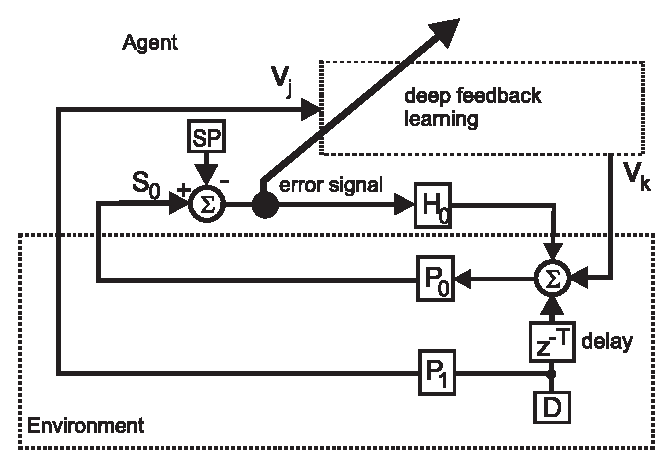
\includegraphics[width=0.75\columnwidth]{closed_loop}
  \caption{A closed loop system with a setpoint $SP$, transfer function $H$ and the
    environment $P_0$ which needs to work against unpredictable disturbances $D$.
    The error signal tunes a deep neuronal network, which has inputs
    $v_j$ that predict the disturbances. The network tries to pre-empt these
    disturbances and generate an appropriate action $v_k$.
    \label{closed_loop}}
\end{figure}

\section{Closed loop learning}

Deep feedback learning operates in a closed loop scenario. Before we
describe the algorithm, we need to place it in a closed loop
context. Fig.~\ref{closed_loop} shows the entire closed loop system
with the deep feedback learning as a black box for now. The idea
is that we have a fixed closed loop which is able to fend off
disturbances, such as an unexpected bend on a road or the sudden
appearance of an enemy. This fixed loop then takes appropriate action
to solve this disturbance, e.g. correcting a car's steering, or
aiming towards and shooting an enemy. In formal terms we have a
setpoint $SP$ which compares the input of organism to a desired
input. If the input deviates from the setpoint an action is generated
with the transfer function $H_0$. This action then eliminates the
disturbance $D$ and arrives via the environmental transfer function
$P_0$ at the input again; thus, the loop is closed. However, we are
not so much interested in the design of the closed loop
but that it generates an \textsl{error signal}. This error signal is
non-zero if a disturbance has happened, and can be
used to tune our deep feedback learning network.

The deep feedback learning network receives additional inputs which are able
to predict the disturbance, and thus prevent the trigger of the feedback
loop. These additional inputs are provided via the transfer function $P_1$
and represent the disturbance in a filtered form. For example a video camera
can provide images of the road ahead, or that of an enemy. Deep feedback
learning has the task to take the error signal and tune its network
to generate an action to minimise the error. In the next section
we describe the deep feedback learning and how this can
compute the appropriate output. Note that deep feedback learning only knows if it has been
successful once its actions have travelled through the environment. Thus learning
evaluates if certain inputs to its network can be used to generate
appropriate actions and these are then slowly transformed into actions.
For that reason the error signal is propagated in a \textsl{forward} fashion
through the network.

\begin{figure}[h!]
  \centering
  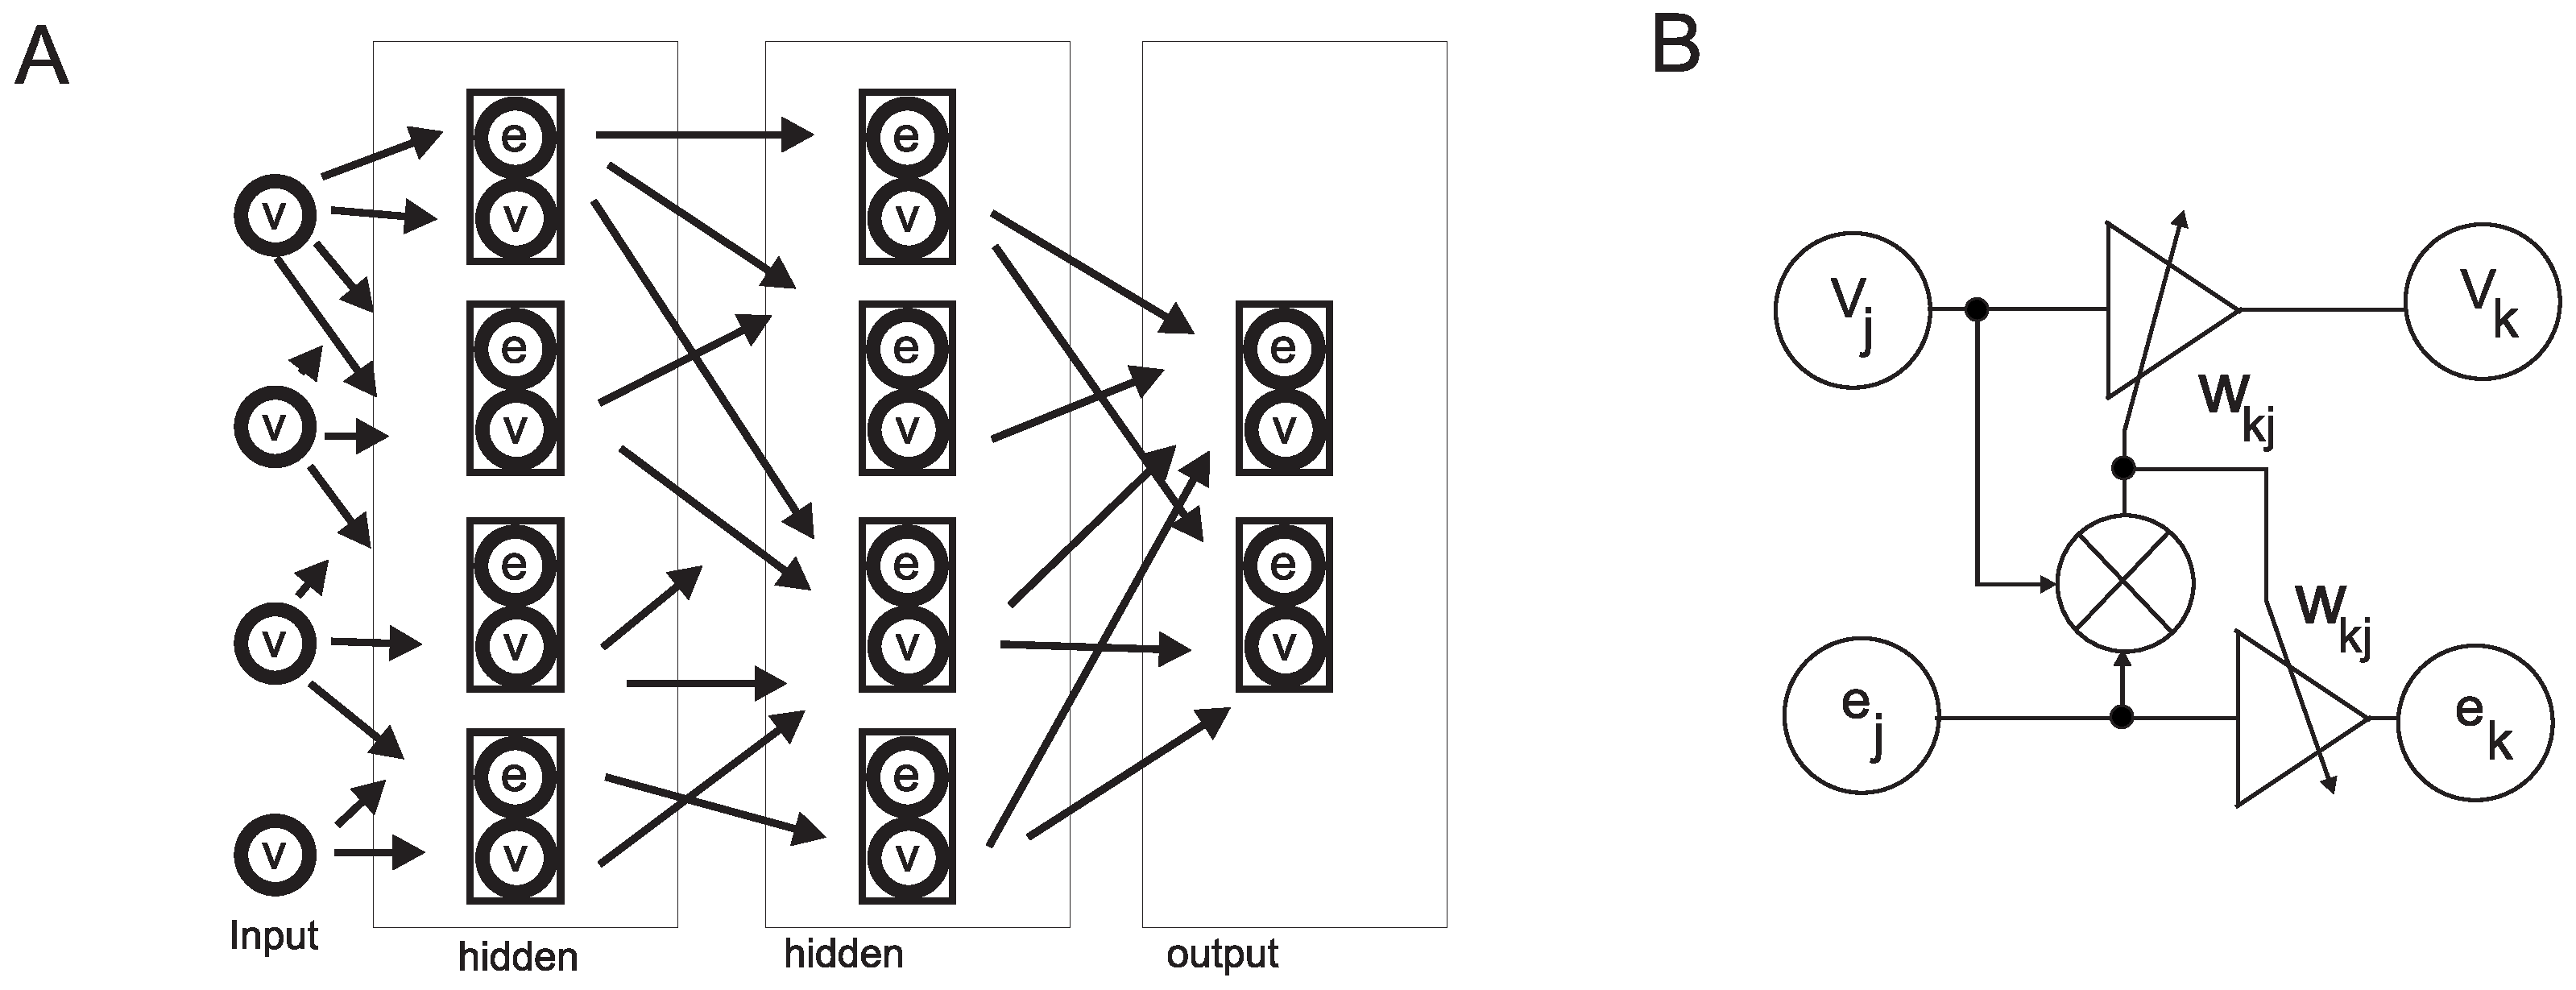
\includegraphics[width=\columnwidth]{netw_together}
  \caption{A) Network overview. Except for the input layer, every
    neuron is a composite cell with an activation $v$ and an error
    term $e$. These are propagated through the network in a weighted
    fashion in parallel.  B) Computation in a single composite cell.
    The presynaptic activities $v_j$ and error signals $e_j$ are used
    to perform correlation based learning and change the weight
    $w_{kj}$ which weights for both activity and error towards the next
    layer.\label{netw_together}}
\end{figure}


\section{Deep feedback learning}
We define a network with an input layer, hidden units and an output
layer which can all have different numbers of neurons (see
Fig~\ref{netw_together}A). In contrast to traditional
networks, every layer (except for the input layer) consists of two
summation nodes: the actual activity and an error signal. These
are processed in two parallel streams.

Let us first focus on the network activity. We
define a multi-layered network, where every neuron is a standard
computational unit that calculates a weighted sum $v_k$ of its inputs $v_j$ and
then applies an activation function $\Theta(v) = \tanh(v)$:
\begin{equation}
  v_k = \Theta\left( \sum_j w_{jk} v_{j} \right) \label{act_sum}
\end{equation}
where the activity flows from neurons in layer $v_j$ to neurons in
layer $v_k$ multiplied by the wegights $w_{jk}$, and then this
is repeated in the next layer. This means for a network with
$N$ layers we have $N-1$ sets of weights $w_{jk}$.

The weight changes are then updated in a semi-Hebbian fashion:
\begin{equation}
  w_{jk}(t+1) = w_{jk}(t) + \gamma v_j(t)  e_k(t) \label{learningRule}
\end{equation}
where $v_j(t)$ is the presynaptic activity and $e_k(t)$ is an error signal
attached to the postsynaptic neuron, so the correlation is
calculated between input signals and the error signal. This is
similar to Hebbian learning except the presynaptic term is the
activity and postsynaptic one is an error signal. The learning rate is $\gamma$.


We now describe the error signal propagation. As outlined above, the
error signal emerges from the feedback loop, and is injected into the
network at its 1st hidden layer as the ``postsynaptic'' activity. The
weight change for this 1st layer can then be calculated directly with
Eq.~\ref{learningRule} by setting $e_k$ to the error signal of the
feedback loop (see Fig.~\ref{closed_loop}).

For the deeper layers, the error signal is computed as a weighted
sum of the error signals from the previous layer:
\begin{equation}
  e_k = \frac{\left( \sum_j w_{jk} e_{j} \right) \Theta^\prime (v_k) }{\sqrt{\sum_j w_{jk}^2}}
\end{equation}
where the $\Theta^\prime (v) = 1 - v^2$ is the derivative of the activation
function $\Theta(v)$: this limits learning when the unit approaches saturation,
as in backprop. The normalisation by the Eucledian weight
distance guarantees that the error propagates through all layers and
not vanishes from layer to layer due to small weights.

A simplified data flow diagram of the learning performed in each layer
is shown in Fig~\ref{netw_together}B, where we see the two processing
streams: both the activity $v_j$ and error signal $e_j$ are
weighted by $w_{jk}$, and summed separately in the next layer.
Remember that for the 1st hidden layer, the error signal is just the
error signal directly injected from the feedback loop. The diagram omits the error
normalisation, scaling and activation derivative in order to focus on the main point that learning happens between the error signal and the
presynaptic activity.

Learning is then performed in three steps: first the activity is
propagated through the network, then the error signal is propagated
via the same mechanism, and finally the weights are adjusted. Thus,
both the error signal and the activity is propagated in a forward
fashion.  Learning itself is ``Hebbian'' but operates by correlating
the actual activation and the error signal.

\begin{figure}[h!]
  \centering
  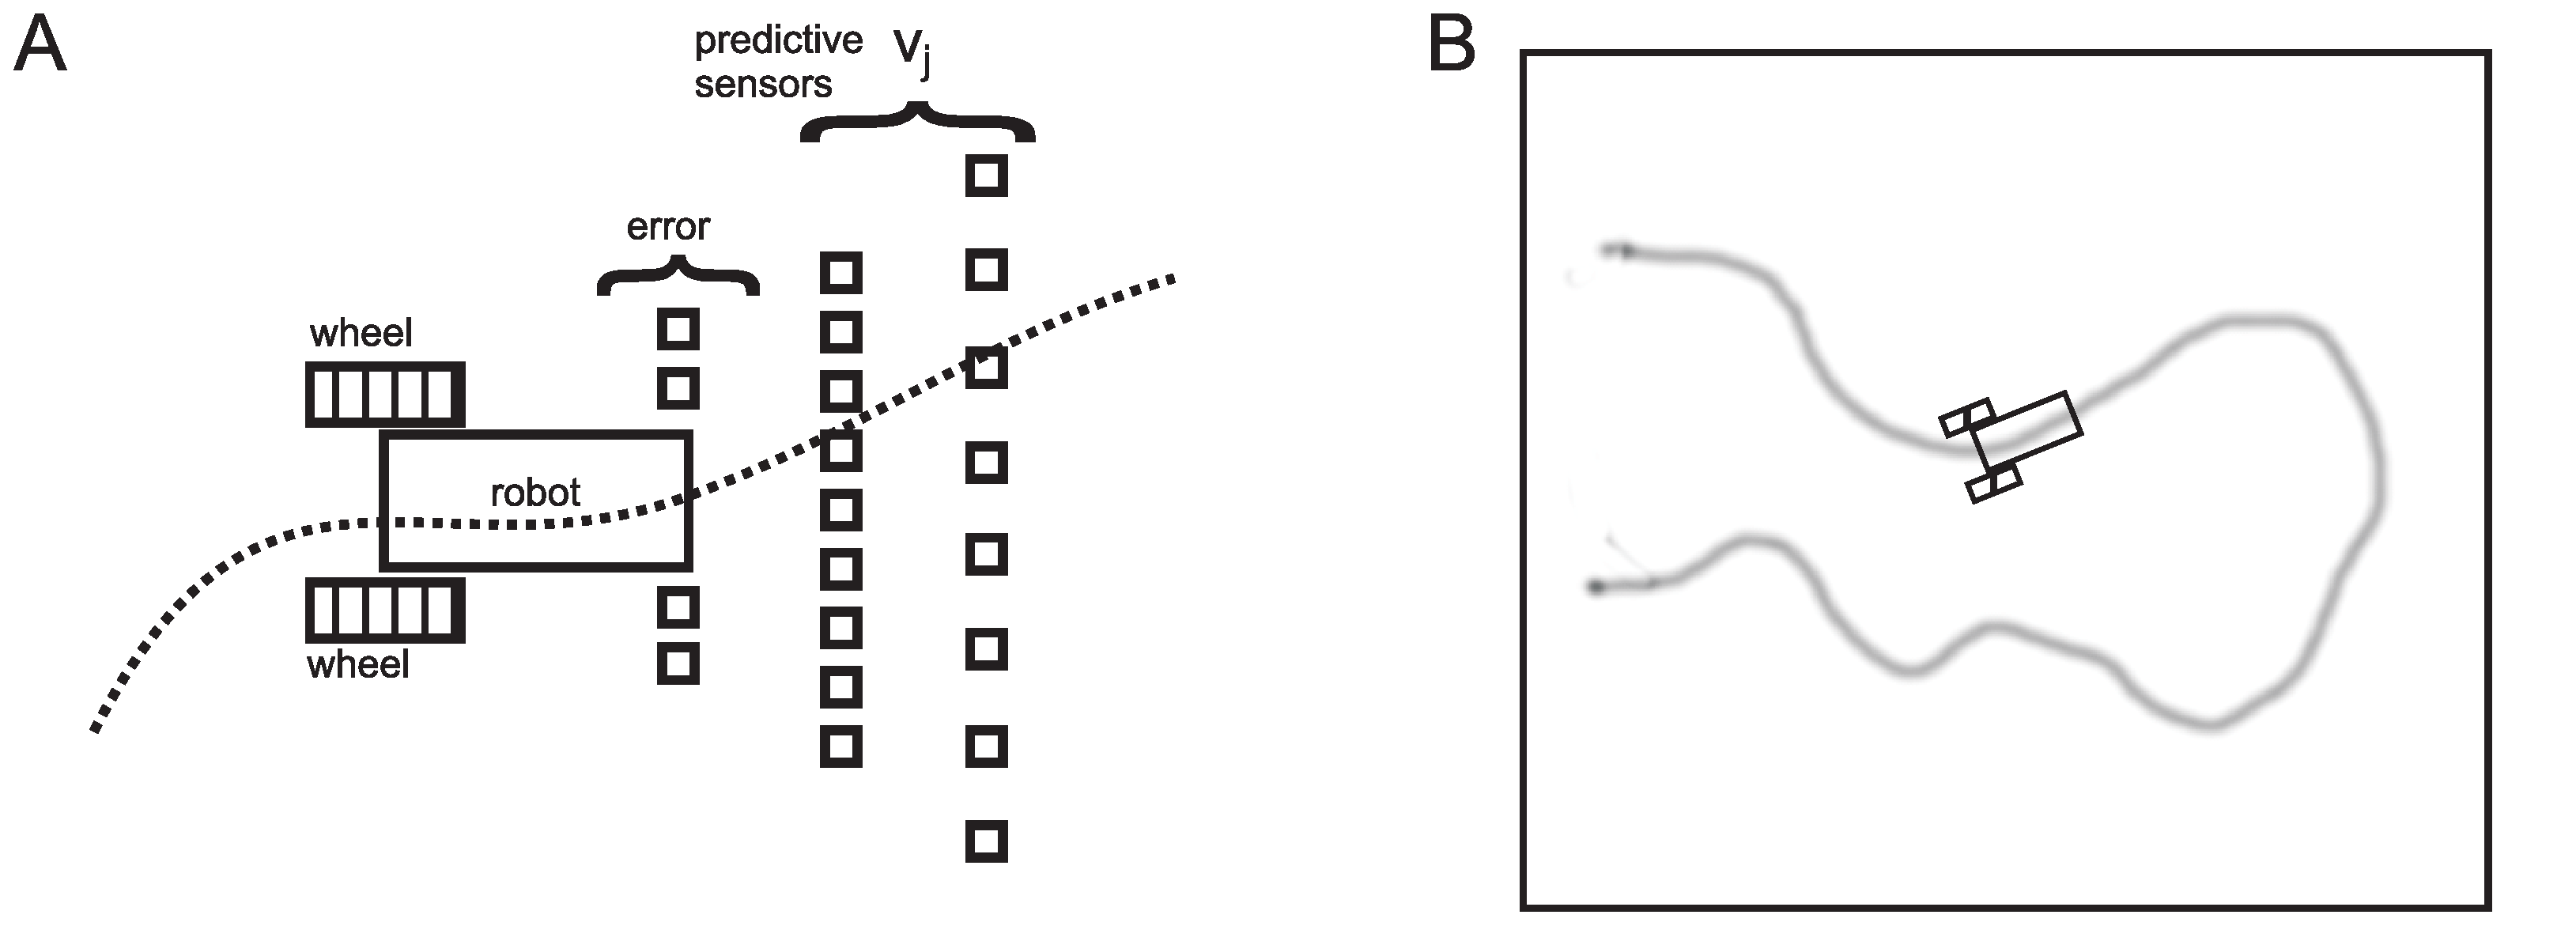
\includegraphics[width=\columnwidth]{linefollower_robot_playground}
  \caption{A) Robot setup. The robot is simulated with a updated
    version of enki for QT5 (https://github.com/berndporr/enki)
    where the line follower is using just the ground sensors of the
    robot to create the error signal ($g_l$, $g_r$) and the predictive signals ($p_m$)
    for DFL. Each of the 30 predictive signals $p_m$ from the two rows of ground sensors
    is split up into 10 2nd order lowpass filters with impulse responses
    lasting from $2$ timesteps to $30$ timesteps and then all feed into the DFL
    network as predictive inputs $v_j$, giving 300 inputs in total.
    The robot has two wheels whose speed is controlled
    by the feedback control and DFL.
    B) The line following scenario used for the simulations. The robot
    attempts to drive along the line and is reversed at the end of the
    line and then drives back. If it hits the boundaries of the playground
    it is also turned around.
    \label{linefollower_robot_playground}}
\end{figure}




\section{Line follower}
In order to demonstrate DFL we need a simple closed loop scenario
which can be improved with the help of an adaptive network.
Fig.~\ref{linefollower_robot_playground} shows a simple line following
robot which has the task of following the line depicted in
Fig.~\ref{linefollower_robot_playground}B to the end, where it
reverses and drives back, and so on. The four ground sensors in
Fig.~\ref{linefollower_robot_playground}A left/right on either side
of the robot create an error signal:
\begin{equation}
\mathrm{error} = (g_{l_1}+2 g_{l_2})-(g_{r_1}+2 g_{r_2}) \label{line_error}
\end{equation}
this error directly creates a steering reaction from the fixed
feedback loop by controlling the speed of the wheels.

The DFL learning circuit uses the predictive ground sensors - these
are first filtered by a Filterbank, which smears them in time and
creates a temporal overlap with the error signal. These filtered
signals are then presented to the $v_j$ of the input layer (see
Eq.~\ref{act_sum}). We have two rows of sensors, one directly in front
of the robot and one which looks further ahead. There are 30 ground
sensors each filtered by 10 filters, giving 300 inputs in total.

The output layer of our deep feedback learner consists of 6 neurons
with activations $v_k$ ($k=0 \ldots 5$) - these can be seen as soft
decision-making units where 3 of them determine the change of speed of
the right wheel, and 3 the left wheel. This leads to the
final formulas for the motor outputs:
\begin{eqnarray}
  \mathrm{leftSpeed} &=& s_0 + \underbrace{g\, \mathrm{error} + \left( 50 v_0 + 10 v_1 + 2 v_2 \right)}_{v_l} \\
  \mathrm{rightSpeed} &=& s_0 - \underbrace{g\, \mathrm{error} + \left( 50 v_3 + 10 v_4 + 2 v_5 \right)}_{v_r}
\end{eqnarray}
where $v_0, \ldots, v_5$ are the 6 outputs from the DFL network. Note
that neither inputs nor outputs are organised in a topographically
meangingful way. The network must discover from the error signals
which sensor inputs $v_k$ will eventually lead to appropriate steering
actions. At the start the network is initialised with random values.

As performance criterion we use the squared average of the error from
Eq.~\ref{line_error}:
\begin{equation}
  \mathrm{error}_\mathrm{avg} =  \mathrm{error}_\mathrm{avg} + 0.001 (\mathrm{error} - \mathrm{error}_\mathrm{avg}) 
\end{equation}
\begin{equation}
  \mathrm{error}_\mathrm{sq} =  \mathrm{error}_\mathrm{avg}^2 \label{line_sqerr}
\end{equation}
As learning tries to minimise the average error, $\mathrm{error}_\mathrm{avg}$ should reach zero in an ideal
scenario. Realistically, driving will never be 100\% perfect, and $\mathrm{error}_\mathrm{avg}$
will stabilise at small values.


\begin{figure}[h!]
  \centering
  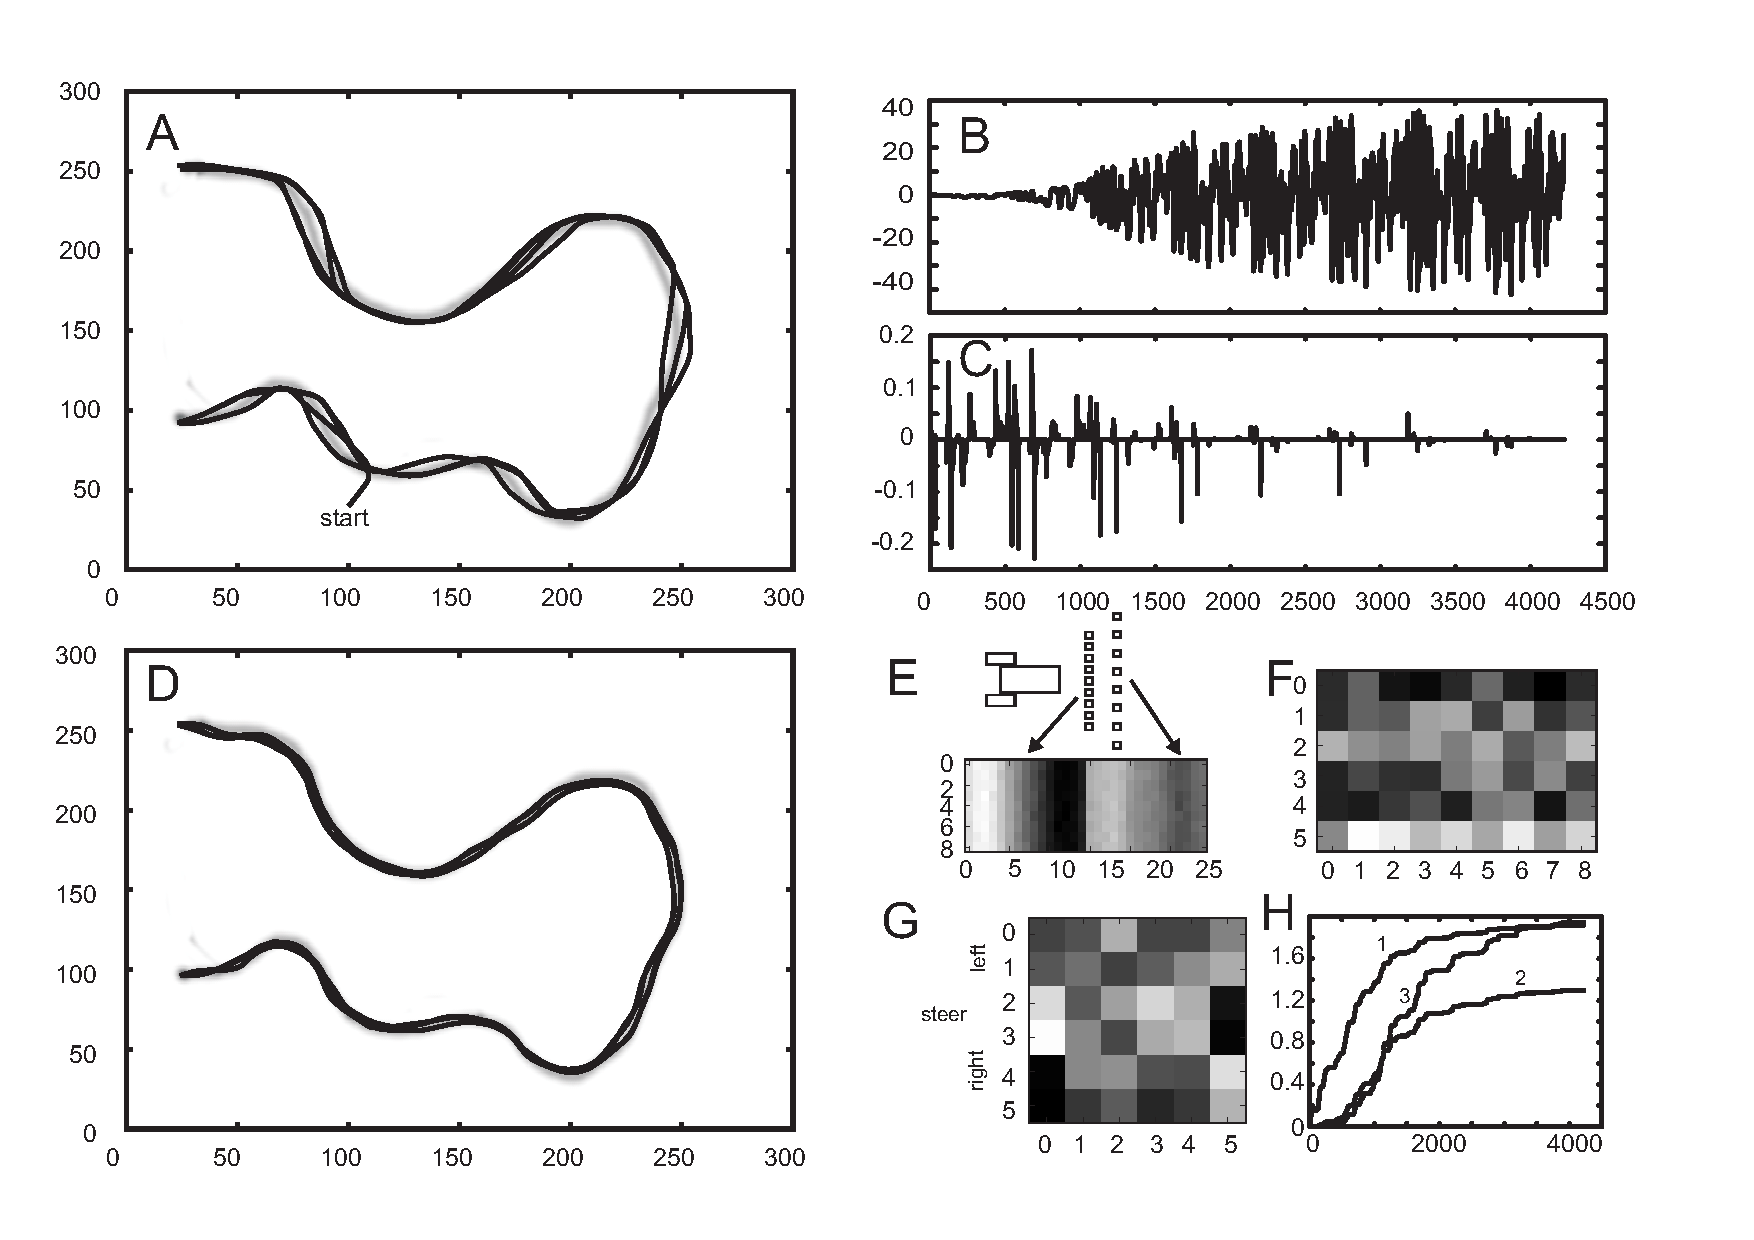
\includegraphics[width=\columnwidth]{line_results}
  \caption{Results of the linefollowing task. A) shows the robot at
    the very start of the simulation run from time step 0 to 600.
    B) the difference between the robot wheel speeds just for the learned
    actions (i.e. the output of the DFL network): $v_l-v_r$.
    C) the error signal squared: $\mathrm{error}_{sq}$.
    D) simulation run just before the end at 13400 to 14000 time steps.
    E-G show the weights of the different layers. The input neurons are on the x-axis
    and the output neurons are on the y-axis.
    E) the weights of the 1st layer, F) the weights of the 2nd layer and
    G) the weights of the output layer.
        H) shows the euclidean distance of the weights for each layer from their initial starting point.
    \label{line_results}}
\end{figure}



\subsection{Results}
Fig.~\ref{line_results} shows the results of a simulation run. In the panels
A) and D) we see the trajectory of the agent over the course of 11400 time steps 
of learning. While in A) the agent clearly
just follows the reflex reaction, leading to large deviations from the track,
in D) the agent follows closely the track and the deviation is minimal --
learning has been successful. In B) we see the network learning the steering actions that keep the agent closely on track.
It can be seen that the network clearly slows down in the change of output.
C) shows the squared error quickly dropping to near zero, leaving only small 
components remaining. E) is the final weight matrix of the 1st layer after learning, 
which correlates the error with the two rows of
predictive ground sensors $v_j$. F) is the weight matrix of the hidden layer and G)
of the output layer. H) shows the Eucledian distance of the
different layers from their starting point. Remember that learning is
always on and the learning rate is 0.0001 for this run.

Overall Fig~\ref{line_results} shows that the network learns to use
the predictive signals from the sensors in front of the robot to
generate its steering output. This steering output slowly becomes
stronger and then stabilises.

The squared average error in Fig.~\ref{line_results}C slowly decays
leaving only small spikes remaining. This is mainly because
the robot is not able to learn one of the steeper bends (see
coordinate 120x50 in D); this causes a spike in the error and
then the robot overcompensates, causing learning in the
other direction and so on.

The weights of the different layers are shown in
Fig.~\ref{line_results}E-G.  The weights in the input layer
(Fig.~\ref{line_results}E) show a slow gradation  from left to right as
expected. Recall that there are two rows of predictive ground
sensors in front of the robot which cause two different weight maps
which can clearly be seen. The inputs 0 to 14 correspond to the near
ground sensor, and 15 to 31 the far sensor which looks further ahead, 
helping the robot predict bends better. These feed then into the 
hidden layer Fig.~\ref{line_results}F
and from there into the output layer Fig.~\ref{line_results}G.

The overall weight development per layer over the time 
is shown in Fig.~\ref{line_results}H. It's interesting to note
that the input layer learns fastest and its weights converge
quickest, while the output layer learns at the slowest rate. Recall 
that the error signal is weighted by the weights for the deeper
layers, but also normalised so that learning happens at about the
same rate in every layer. However, the deeper layers show more
of an exponential growth. The weights grow at a slower
and slower pace but still continue because the robot is not able to completely
avoid its reflex, and also probably because the system is non-linear.
However, the error is very low even when the weights still change
substantially; one could switch off learning if early stability
is required.



\begin{figure}[h!]
  \centering
  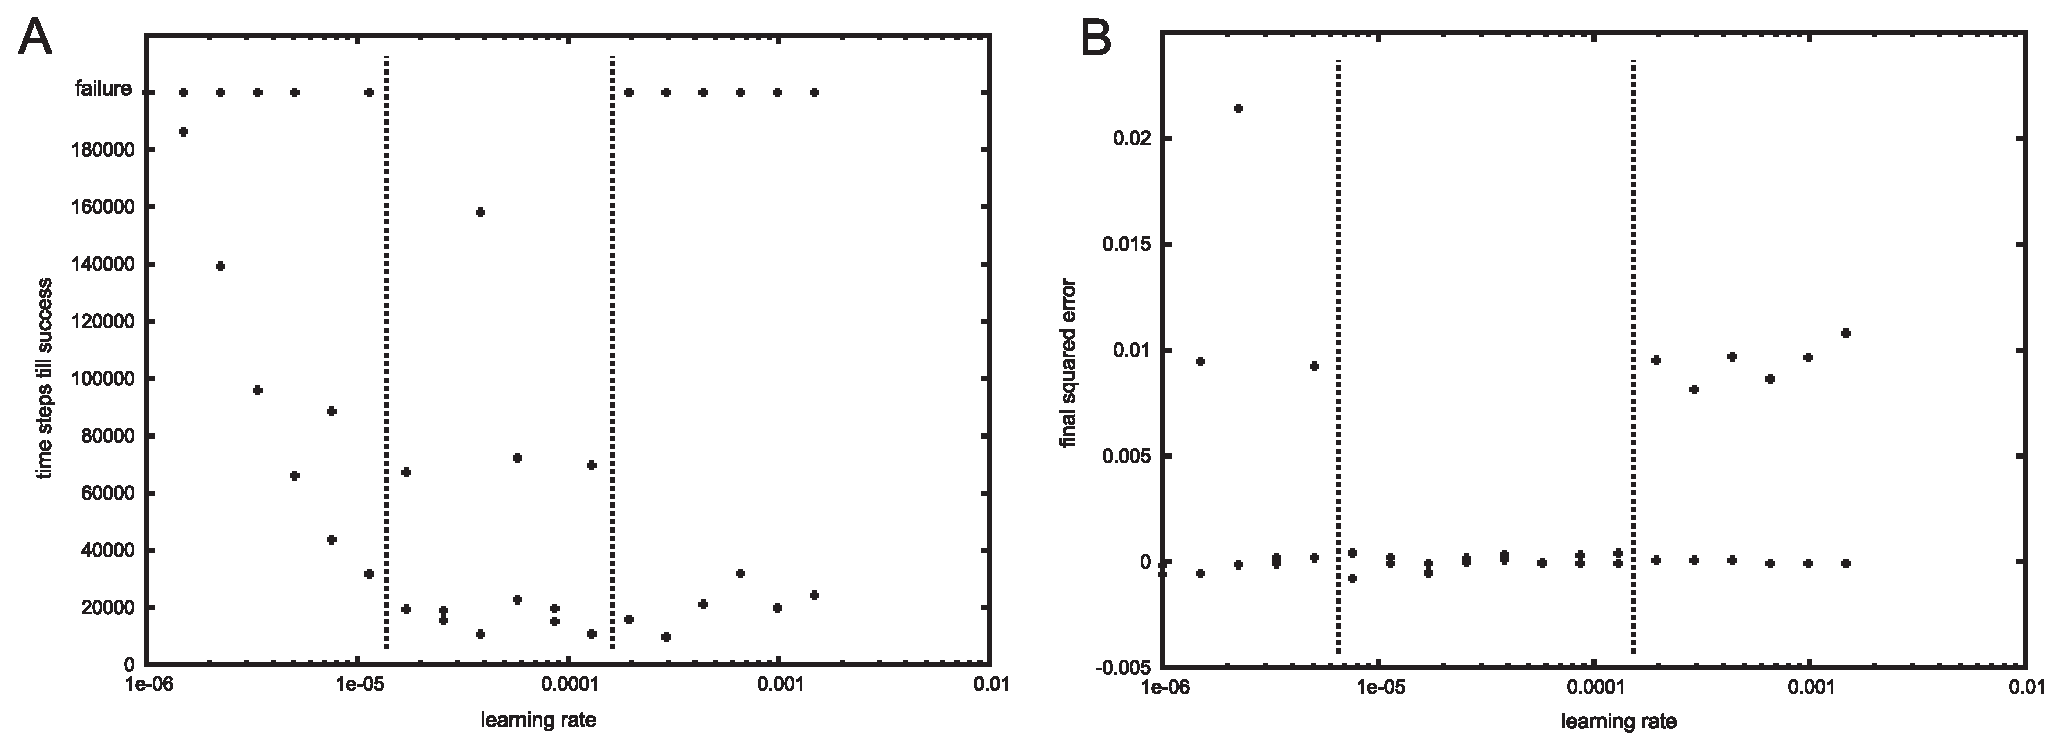
\includegraphics[width=\columnwidth]{line_stats}
  \caption{Statistics of the line following task. A) shows the relation between
    simulation steps against learning rate. For every learning rate two runs have
    been conducted with different random number seeds to test the dependence on the
    initialisation of the weights. The simulation was marked successful if the
    squared error Eq.~\ref{line_sqerr} stayed below $10^{-6}$ for more than $2500$
    timesteps. The simulation was aborted after $200,000$ time steps if this criterion
    hasn't been reached. Between the dotted lines every run has been successful.
    B) shows the final squared error for different learning rates and again between
    the dotted lines we have runs which resulted in low squared errors.
    \label{line_stats}}
\end{figure}

We have run statistics of the line follower where we varied the
learning rate over 4 orders of magnitudes and evaluated how long it
takes to stay below a certain error threshold for a specified time
(Fig.~\ref{line_stats}A), and the resulting squared error
(Fig.~\ref{line_stats}B). The time to reach the criterion decreases
with higher learning rates and is stable between learning rates of
approx $10^{-5}$ and $10^{-4}$, i.e. about one order of
magnitude. Each simulation was run twice with different random seeds
to test for initialisation effects. In the stable
region this results in different times until success, whereas outwith
this region about half of the runs fail. For lower learning rates the
trial might still succeed in the end, e.g. Fig.~\ref{line_stats}B
shows only three runs with low learning rates not converging. At low
learning rates the robot sometimes learns essentially ``open loop''
with the error signal having very little impact, and learning can
drift very slowly in the wrong direction only to be corrected later.
At very high learning rates we get essentially one shot learning,
which might learn accidentally the wrong behaviour. In the
optimal regime (between the dotted lines) learning always arrives at low
error values. Overall it's interesting that lower learning rates
aren't neccessarily better, but rather that intermediate learning
rates perform best as they combine both, learning fast but slow enough
so that the error signal can correct mistakes.




\section{Shooter game}
In this scenario, we try to learn to play a first-person shooter
purely from visual inputs. We use the Vizdoom
(http://vizdoom.cs.put.edu.pl/) environment for this purpose, and
train a controller to play against a single pretrained bot from Intel
that ran in the Vizdoom 2016 competition. The setup was as follows:

The images returned from Vizdoom are RGB 160x120. We rendered the
enemy in blue, and formed a reflex signal by finding the bounding box
of the pixels closest to that colour. Note that the reflex is slow and is
inherently noisy, as other events in the game are also rendered blue
(e.g. the ‘flashes’ that happen at respawns). The reflex also fails at
times when the enemy is too distant or too close to the camera. For
learning, we only supply the network with the greyscale image
(Fig.~\ref{shooter_results}G) flattened into a vector of $19200$
inputs, so it is forced to discover purely spatial cues. The reflex is
computed relative to the image centre, so a negative value implies the
enemy is on the left. Shooting behaviour is entirely hardwired: if an
enemy is detected within a threshold of the image centre, the bot
fires. Note that the bot's only actions are to rotate in the plane,
and shoot. Instead of separate outputs for left and right, we have a
single value produced by 3 neurons acting at different sensitivites:
\begin{equation}
\Delta \theta = g_{err}\, \mathrm{error} + g_{net} \left( 10 v_0 + 3 v_1 + v_2 \right)
\end{equation}
where $v_0, \ldots, v_2$ are the network outputs, and $\Delta \theta$ is the change in orientation.


\begin{figure}[h!]
	\centering 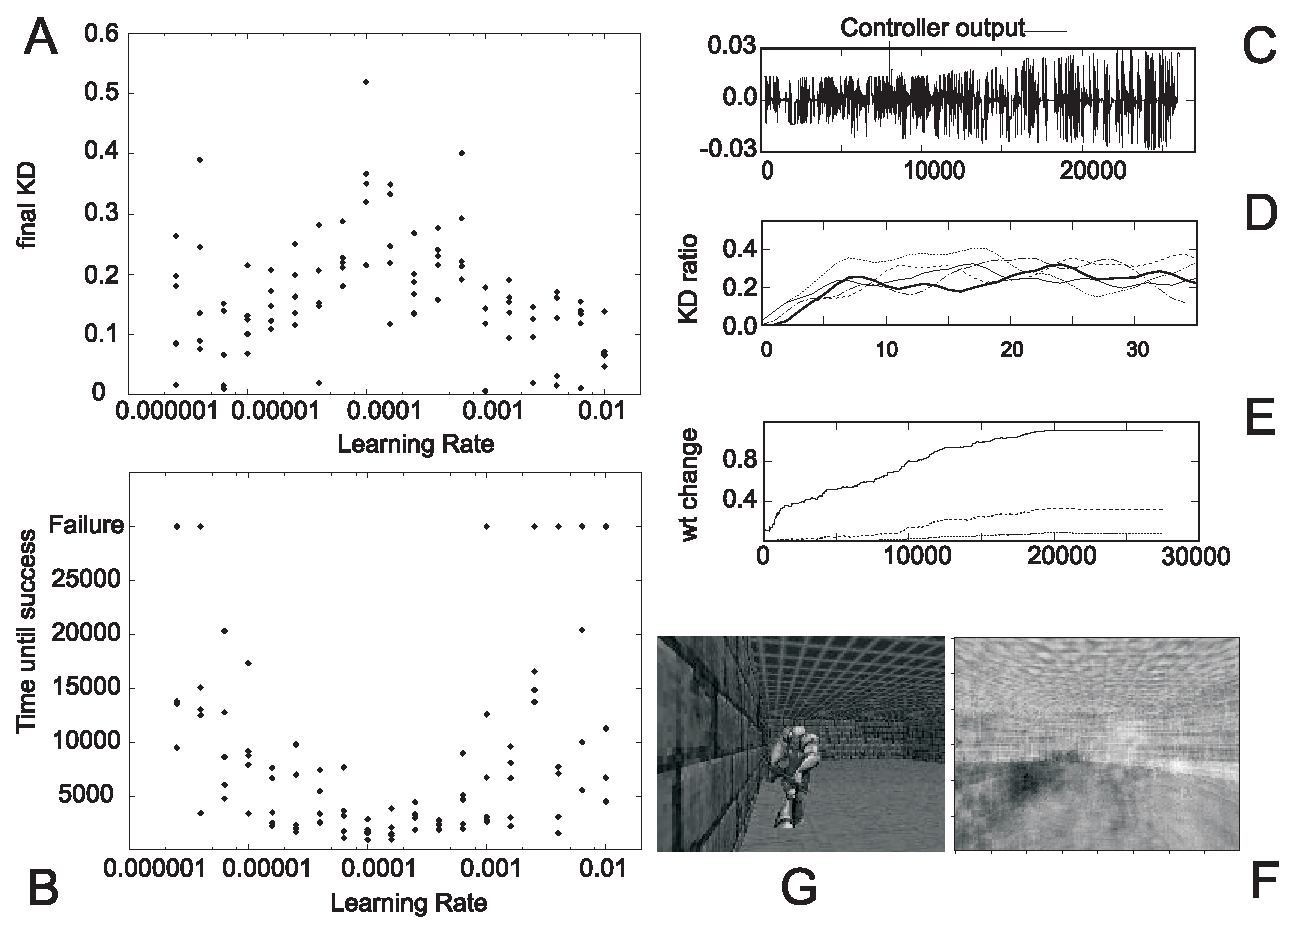
\includegraphics[width=\columnwidth]{FPSFig7}
	\caption{A) KD at end of trial. B) Time to success vs learning
          rate - success is if the smoothed KD ratio reaches a threshold of 0.15. C) $\Delta \theta$, the change in bot's orientation over time, purely from the DFL output, in arbitrary units. D) KD learning curves - the time series of kills/deaths is filtered with a 2nd order lowpass filter to get a moving average, plotted against kill event number. E)
          Euclidean distance of weights for each layer from their initial point, against learning step. F) Example input weights. G) Example input frame.
		\label{shooter_results}}
\end{figure}

\subsection{Results}
As before, we see that the controller outputs steadily increase over
time (Fig.~\ref{shooter_results}C). With a high value of $g_{net}$,
the bot can make very rapid aiming movements. This has the advantage
that the error can in principle be reduced very quickly; it also
causes the bot to sometimes make large rotations even when the enemy
is out of the field of view, which helps with exploration. On the
other hand, it can cause the aiming to overshoot and oscillate around
the target.  The weights grow in a similar pattern to before, although
their progression is less smooth, due to the more discontinuous nature
of the error signal (Fig.~\ref{shooter_results}E). The different scales are likely due to the inputs having 

Unlike the Line Follower, it is not possible here to drive the error
to zero, as there are discontinuities when either bot respawns, and so
the enemy will often abruptly appear somewhere in the image. One
performance measure is simply how often our bot is killed vs how often
it kills the enemy. In gaming, this is called the kill/death ratio,
and we plot some smoothed KD curves in Fig.~\ref{shooter_results}D. To
do statistics, we measure the time taken to reach a threshold KD (0.15) -
Fig.~\ref{shooter_results}B shows this as a function of learning
rate. As before, there is a stable region in the middle where learning
is consistently successful. We also plot the smoothed KD for the final
step of each trial(Fig.~\ref{shooter_results}A); although a noisy
measure, the same pattern emerges. Over time, the input weights blur
the background, leaving dark and light blobs to detect the enemy and
generate an aiming response (Fig.~\ref{shooter_results}F).

Note that this is only one skill of a functioning FPS bot, as that would
require additional skills such as seeking rewards (e.g. finding health packs) and
navigating the environment (e.g. avoiding collisions). Future research
will investigate whether the DFL approach can be used to acquire such
skills, using the same fundamental approach of learning to anticipate
a prewired behaviour.


\section{Discussion}
We have shown that a deep network which propagates its errors in a forward
fashion from its inputs to its outputs is able to solve closed loop
learning tasks. We have demonstrated this in both a first person
shooter and a driving scenario.

Closed loop learning which aims to maximise a function or minimise one
is usually referred to as reinforcement learning, where an agent learns to
navigate an action space in a way that it maximises its accumulative
reward \cite{Dayan1992}. The main drawback of this approach
is the discrete state space which makes it hard to solve analogue
problems. To overcome this problem, closed loop learning rules using
correlation-based techniques \cite{Verschure98summary} were introduced.
These networks perform well in real robot tasks but are usually restricted to 
simple network architectures. DFL addresses this
deficiency by introducing a deep architecture but staying firmly
on correlation-based territory.

Plasticity has always been hotly debated in neurophysiology -- the
general understanding is that a large postsynaptic Calcium
concentration causes LTP \cite{Malenka99,Bennett2000} and a low one
causes LTD \cite{Mulkey1992}. This requires a strong pre-synaptic
drive to achieve a strong postsynaptic activity, and with that Ca
influx \cite{Meunier2017}. In mathematical terms this would just lead
to self-amplification of the synaptic weight, where strong presynaptic
activity would lead to more postsynaptic activity and in turn stronger
weights, and so on. However, suppose the learning signal and the
actual activity were transmitted via the same synapse but
fundamentally separated \cite{Lindsay2017}, for example by using
different frequencies: high frequency potentials could cause
plasticity changes while low frequency potentials propagate behaviourally
relevant activity \cite{Canolty2010}. In this way one could still use Hebbian
plasticity but without its detrimental autocorrelation term, because the
correlation would be between two different signals.

A different stance about synaptic plasticity (and ultimately how
autonomous agents learn) has been taken by the deep learning community
which recently claimed that error backpropagation is biologically
realistic \cite{Lillicrap2016,Roelfsema2018}. This has been
demonstrated in a network with one hidden layer by introducing a
separate feedback pathway from the output of the network to this
hidden layer. While this shows promising results it still operates in
an open loop fashion (i.e. output control), and thus contradicts the
requirement for an agent to control its inputs, which leads to a
discussion about closed loop learning.

Autonomous behaviour can only be understood by observing the whole
loop \cite{Porr2005kyb}, be it reinforcement learning \cite{Sutton98}
or correlation based learning \cite{Verschure91}. Of course not all
feedback loops traverse through the physical environment; they could
be efference copies \cite{Uexkuell26,Graesser86} or gating signals
which are presented to minimise errors. However, even these signals
need to be evaluated at the input of the agent, for example when
stabilising an input image, the goal is itself an image, and therefore
an input and not an output.

Given that in DFL the error is propagated from the input to the output
the novel aspect is that the more layers DFL has, the more it is remote
from the immediate error feedback. This allows for flexibility which
can be tuned by the number of layers, and demonstrates that the agent
performs input control. The actions can be substantially varied as long as
the error signal can be minimised and will be more pronounced with
more hidden layers. In other words the more hidden layers we have the
more behavioural flexibility the agent will achieve.






\bibliographystyle{splncs03}

\bibliography{hebb,ours,embodiment,laplace}

\end{document}



\begin{figure}[h!]
  \centering
  \includegraphics[width=\columnwidth]{arena_cct.pdf}
  \caption{A. Overview of the simulation environment. The arena has two markers, labelled R and B (red and blue), within   \label{fig:cct}
    }
\end{figure}

